% BHU PYQ -- Professional Exam Template
\documentclass[11pt,a4paper]{article}

\usepackage[a4paper,top=2.5cm,bottom=2.5cm,left=2.8cm,right=2.8cm,headheight=14pt]{geometry}
\usepackage{amsmath,amssymb}
\usepackage[T1]{fontenc}
\usepackage[utf8]{inputenc}
\usepackage{lmodern}
\usepackage{microtype}
\usepackage{fancyhdr}
\usepackage{enumitem}
\usepackage{hyperref}
\usepackage{lastpage}
\usepackage{parskip}
\usepackage{tikz}
\usetikzlibrary{arrows.meta,shapes,positioning}

\hypersetup{colorlinks=true,urlcolor=black,linkcolor=black,
  pdftitle={B.Sc. (Hons.) Zoology Sem-VI ZOB-604 -- BHU PYQ}}

\pagestyle{fancy}
\fancyhf{}
\renewcommand{\headrulewidth}{0.4pt}
\renewcommand{\footrulewidth}{0.4pt}
\fancyhead[L]{\small   \textit{Banaras Hindu University}}
\fancyhead[R]{\small   \textit{Zoology Paper: ZOB-604}}
\fancyfoot[C]{\small Page  \thepage\ of \pageref{LastPage}}


\newlist{parts}{enumerate}{2}
\setlist[parts,1]{label=(\alph*),leftmargin=*,itemsep=4pt,topsep=3pt}
\setlist[parts,2]{label=(\roman*),leftmargin=*,itemsep=2pt,topsep=2pt}

\newcommand{\pts}[1]{\hfill   \textit{[#1]}}


\begin{document}


\begin{center}
  {\large\bfseries BANARAS HINDU UNIVERSITY}\\[2pt]
  {
\normalsize B.Sc. (Hons.) Semester VI Examination, 2022-23}\\[6pt]
  \rule{0.8\linewidth}{0.5pt}\\[6pt]
  {\large\bfseries Zoology}\\[4pt]
  {\large\bfseries Paper: ZOB-604 --- Evolution and Animal Behaviour}\\[4pt]
  {
\normalsize Time: Three hours \hfill Full Marks: 70}
\end{center}

\rule{\linewidth}{0.4pt}

\smallskip



\noindent   \textit{Note: Answer three questions from Section-A (including Question No. 1 which is compulsory) and three questions from Section-B (including Question No. 1 which is compulsory). Use a separate answer book for each section. The figures in the right-hand margin indicate marks.}

\bigskip

\begin{center}
   \textbf{SECTION -- A} \\
   \textbf{(Evolution) (Marks: 35)}
\end{center}




\noindent   \textbf{Question 1.} Answer the following parts:

\begin{parts}
  \item Define the following:\pts{$5  \times 1 = 5$}
  
\begin{parts}
    \item Assortative mating
    \item SNP
    \item Allozyme
    \item Eon
    \item Sympatric speciation.
  \end{parts}
  
  \item Differentiate between the following:\pts{$3  \times 2 = 6$}
  
\begin{parts}
    \item Relative dating and Radioactive dating
    \item Founder effect and Bottleneck effect
    \item Concealing and Alluring mimicry.
  \end{parts}
\end{parts}

\medskip


\noindent   \textbf{Question 2.} Write short notes on the following:\pts{$3  \times 4 = 12$}

\begin{parts}
  \item Tandem repeat polymorphism
  \item The chronological evolution of horse
  \item Natural selection as mode of evolution.
\end{parts}

\medskip


\noindent   \textbf{Question 3.} Giving suitable examples, explain various isolating mechanisms that hinder interbreeding between the species.\pts{12}

\pagebreak

\medskip


\noindent   \textbf{Question 4.} Give a brief account of different types of fossils. Add a note on the significance of fossil study.\pts{12}


\begin{center}

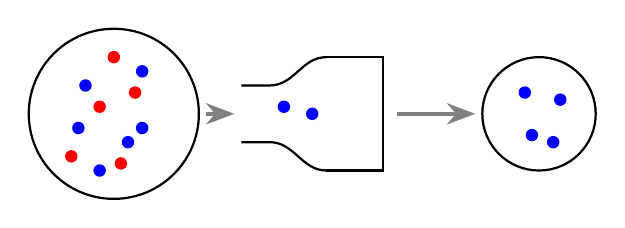
\begin{tikzpicture}[scale=0.9, >=Stealth, every node/.style={font=\small}]
  \draw[thick] (-3, 0) circle (1.2);
  
ode[above=1.2cm] at (-3, 0) {Original Population};
  \foreach \pos in {(-3.4, 0.4), (-2.6, 0.6), (-2.8, -0.4), (-3.2, -0.8), (-2.6, -0.2), (-3.5, -0.2)} {
    \fill[blue] \pos circle (2.5pt);
  }
  \foreach \pos in {(-3.0, 0.8), (-2.7, 0.3), (-3.2, 0.1), (-2.9, -0.7), (-3.6, -0.6)} {
    \fill[red] \pos circle (2.5pt);
  }
  
  \draw[thick] (0, 0.8) -- (0.8, 0.8) -- (0.8, -0.8) -- (0, -0.8);
  \draw[thick] (0, 0.8) to[out=180, in=0] (-0.8, 0.4) -- (-1.2, 0.4);
  \draw[thick] (0, -0.8) to[out=180, in=0] (-0.8, -0.4) -- (-1.2, -0.4);
  
ode[above=0.8cm] at (0, 0.8) {Bottleneck Event};
  
  \fill[blue] (-0.6, 0.1) circle (2.5pt);
  \fill[blue] (-0.2, 0.0) circle (2.5pt);
  
  \draw[thick] (3, 0) circle (0.8);
  
ode[above=0.8cm] at (3, 0) {Surviving Population};
  \foreach \pos in {(2.8, 0.3), (3.3, 0.2), (2.9, -0.3), (3.2, -0.4)} {
    \fill[blue] \pos circle (2.5pt);
  }
  
  \draw[->, ultra thick, gray] (-1.7, 0) -- (-1.3, 0);
  \draw[->, ultra thick, gray] (1.0, 0) -- (2.1, 0);
\end{tikzpicture}
\end{center}

\bigskip

\begin{center}
   \textbf{SECTION -- B} \\
   \textbf{(Animal Behaviour) (Marks: 35)}
\end{center}




\noindent   \textbf{Question 1.} Answer the following parts:

\begin{parts}
  \item State whether the following statements are True or False. Justify your answer in 2-3 sentences each:\pts{$3  \times 2 = 6$}
  
\begin{parts}
    \item A fixed action pattern is a changeable series of actions triggered without any stimulus.
    \item Learned behaviour is inherited, automatic and inflexible.
    \item An animal making new associations between previously learned tasks to solve a new problem is known as latent learning.
  \end{parts}
  
  \item Define the following:\pts{$5  \times 1 = 5$}
  
\begin{parts}
    \item Habituation
    \item Imprinting
    \item Inclusive fitness
    \item Circadian rhythm
    \item Zugunruhe.
  \end{parts}
\end{parts}

\medskip


\noindent   \textbf{Question 2.} Describe the patterns of different social behaviours in animals.\pts{12}

\pagebreak

\medskip


\noindent   \textbf{Question 3.} Answer the following:

\begin{parts}
  \item Write a note on genetic control of behaviour.\pts{6}
  \item Describe different modes of communication in animals.\pts{6}
\end{parts}

\medskip


\noindent   \textbf{Question 4.} Write notes on the following:\pts{$2  \times 6 = 12$}

\begin{parts}
  \item Costs and benefits of group living
  \item Migration in birds.
\end{parts}

\vfill
\rule{\linewidth}{0.4pt}

\begin{center}\small
\href{https://bhu-exam.vercel.app/}{Click Here}\\[4pt]\href{https://me-aryan.vercel.app/}{Click Here}\\[4pt]\href{https://quashan-me.vercel.app/}{Click Here}
\end{center}

\end{document}
